\section{Introduction}

\vspace{2mm}
\noindent \textbf{Machine Learning.} Machine Learning (ML) is revolutionizing many fields.
It is now being used in many domains including e-commerce, web and social media, interactive voice agents, and even in critical applications in autonomous vehicles and healthcare.
From a software systems point of view, ML can be viewed as a flexible framework for solving hard programming problems.
For instance, it is nearly impossible for a software developer to program an object detector that can identify different objects from an image.
But using ML and a sufficient amount of labeled training data, one can \textit{learn a program} to do the same, which can even surpass human-level accuracy.

\vspace{2mm}
\noindent \textbf{Database Management Systems.} Database management systems (DBMSs) are complex software systems that are the result of decades of research and highly-advanced engineering efforts.
They provide declarative and easy to use interfaces for the users to manage the data while handling the complexity underneath.
DBMSs cover the entire vertical spectrum of computing from user interfaces to hardware-level optimizations.
They are at the core of many critical software applications and have also influenced much of the development of other popular data management systems such as NoSQL, Big Data, and Machine Learning Systems.
Out of the many types of database management systems, relational database management systems (RDBMSs) remain the most widely used type.
Thus, for this paper, we primarily focus on RDBMSs.

\vspace{2mm}
\noindent \textbf{ML for DBMSs.} DBMSs are also full of hard to program problems.
Some of these problems include query optimization, physical database design optimization, buffer management, etc.
These problems are hard because generically solving them requires searching over intractable search spaces (e.g., query optimization) or because of the inability to predict the future (e.g., buffer management).
As a result, DBMS developers have to use heuristics, restrict the problem space, or even rely on human intervention (e.g., in knob tuning) to solve these problems.
The goal of these heuristics and restrictions is not to find an optimal solution for a particular instance, but to find a solution which has a safe worst-case performance on all cases.
However, in most cases, it is possible to find a better solution for a specific instance of the problem.
For instance, if we know the set of queries that our DBMS is going to receive, we can develop a dedicated system which works best only for those queries.
But that kind of a solution would require developing custom implementations for each specific case which amplifies the resource costs and also becomes unmanageable at scale such as in the cloud.
Alternatively, ML provides a flexible framework to automatically learn an efficient program to solve these problems for a specific instance without being explicitly programmed by a human developer.

\begin{figure*}
    \centering
    \vspace{-6mm}
    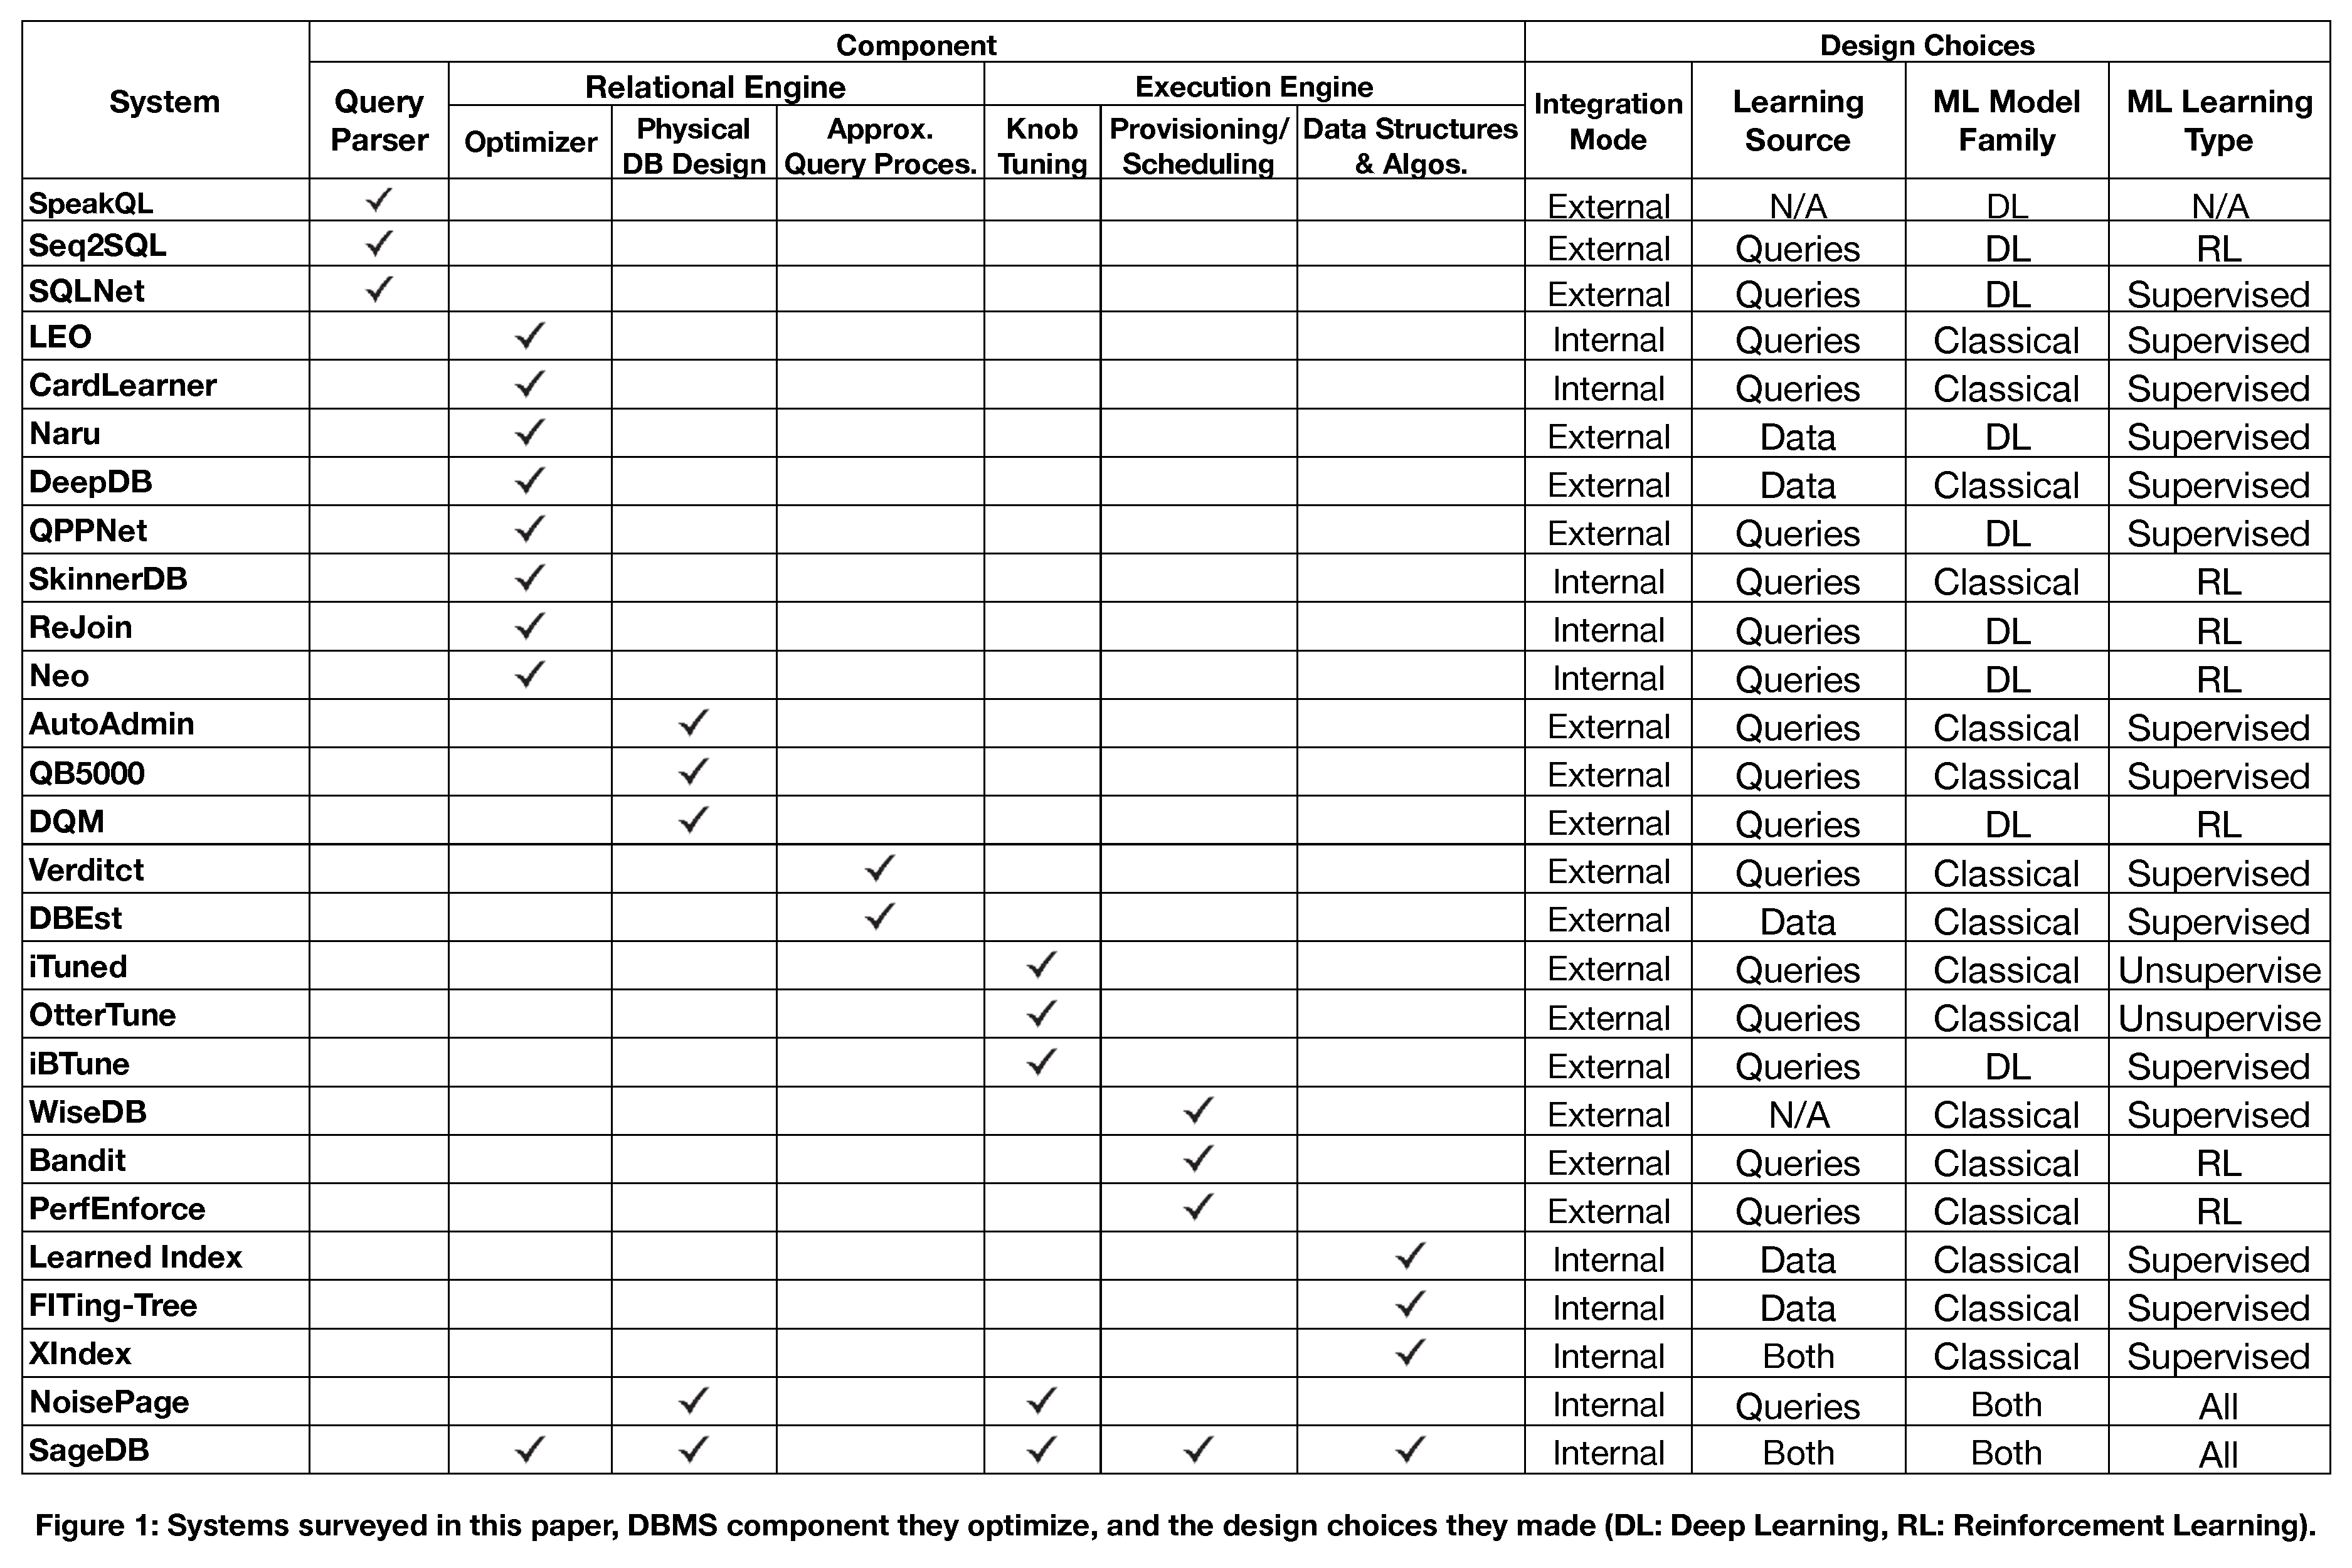
\includegraphics[height=0.85\textwidth, angle=90]{images/taxonomy.pdf}
\end{figure*}

\vspace{2mm}
\noindent \textbf{Our Contribution.} In this paper, we survey the existing landscape of using ML to solve hard programming problems in DBMSs. 
We divide the DBMS into three main sub-components: 1) Query Parser, 2) Relational Engine, and 3) Execution Engine. Some background on each of these sub-components and different ML methods is provided in Section 2.
We then identify several systems that have proposed using ML in Query Parser, Relational Engine, and Execution Engine in Section 3, 4, and 5, respectively.
In Section 6, we identify three overarching design decisions that a DBMS developer has to make when incorporating ML into a DBMS: 1) integration mode, 2) learning source, and 3) choice of ML paradigm, and also discuss the trade-offs of available options.
An abstract summary of where the surveyed systems fall in this taxonomy is presented in Figure 1.
While there are significant accomplishments, the field is still in its infancy, and many challenges remain open.
In Section 7, we identify three such open challenges: 1) improving robustness, 2) rethinking the DBMS architecture, and 3) exploiting transfer learning.